\begin{frame}{Meine Aufgaben}
	\begin{itemize}
		\item Einarbeiten in das Optimal Steps Model
		\item Einbinden der Horse Klasse ins OSM
		\item Erstellen eines Testszenarios 
	\end{itemize}
\end{frame}

\begin{frame}{Optimal Steps Model}
	\begin{itemize}
		\item Nutzenfunktion
		\item Optimization
		\item Update Schemes
	\end{itemize}
\end{frame}

\begin{frame}{Implementierung OSM}
	\begin{figure}
		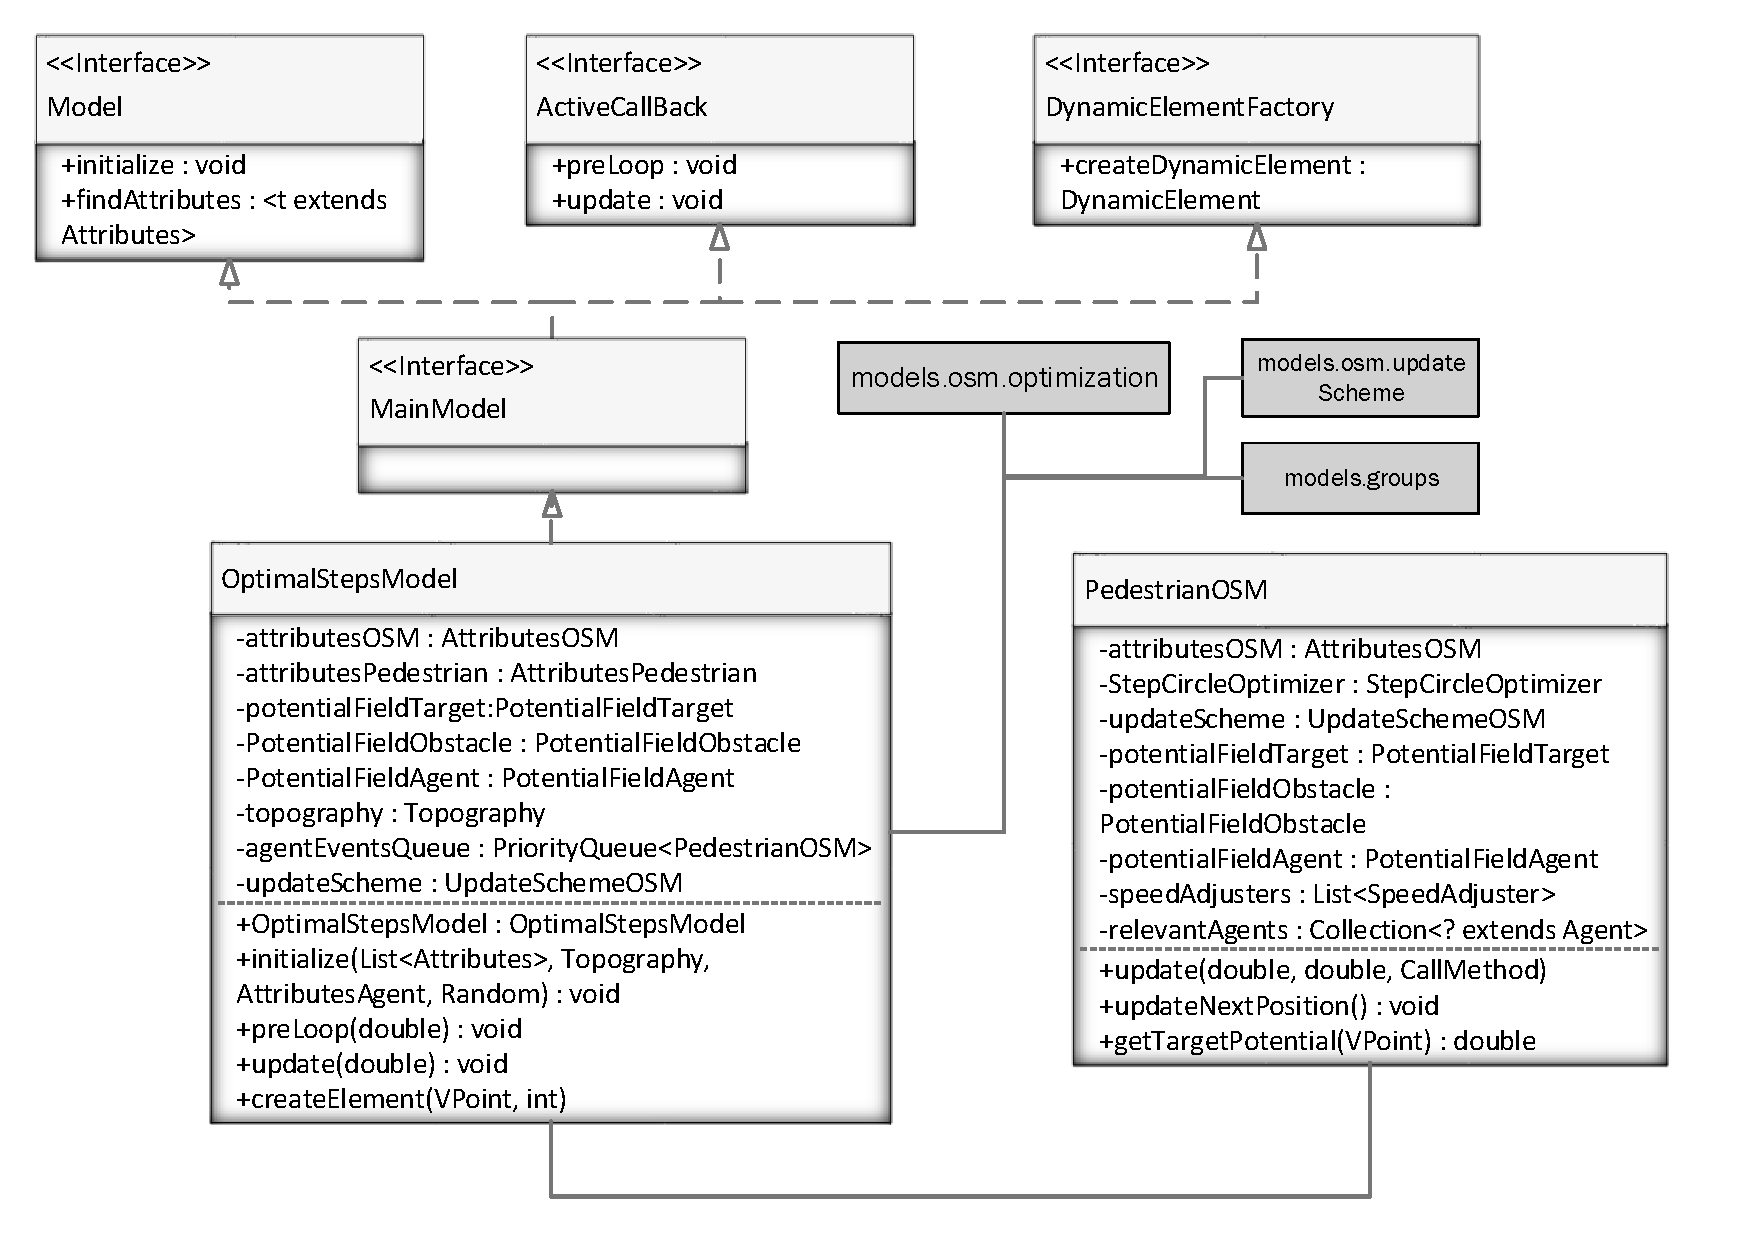
\includegraphics[width=\textwidth, keepaspectratio]{appendix/uml/OSM-vorher.pdf}
	\end{figure}
\end{frame}

\begin{frame}{Implementierung HorseOSM}
	\begin{figure}
		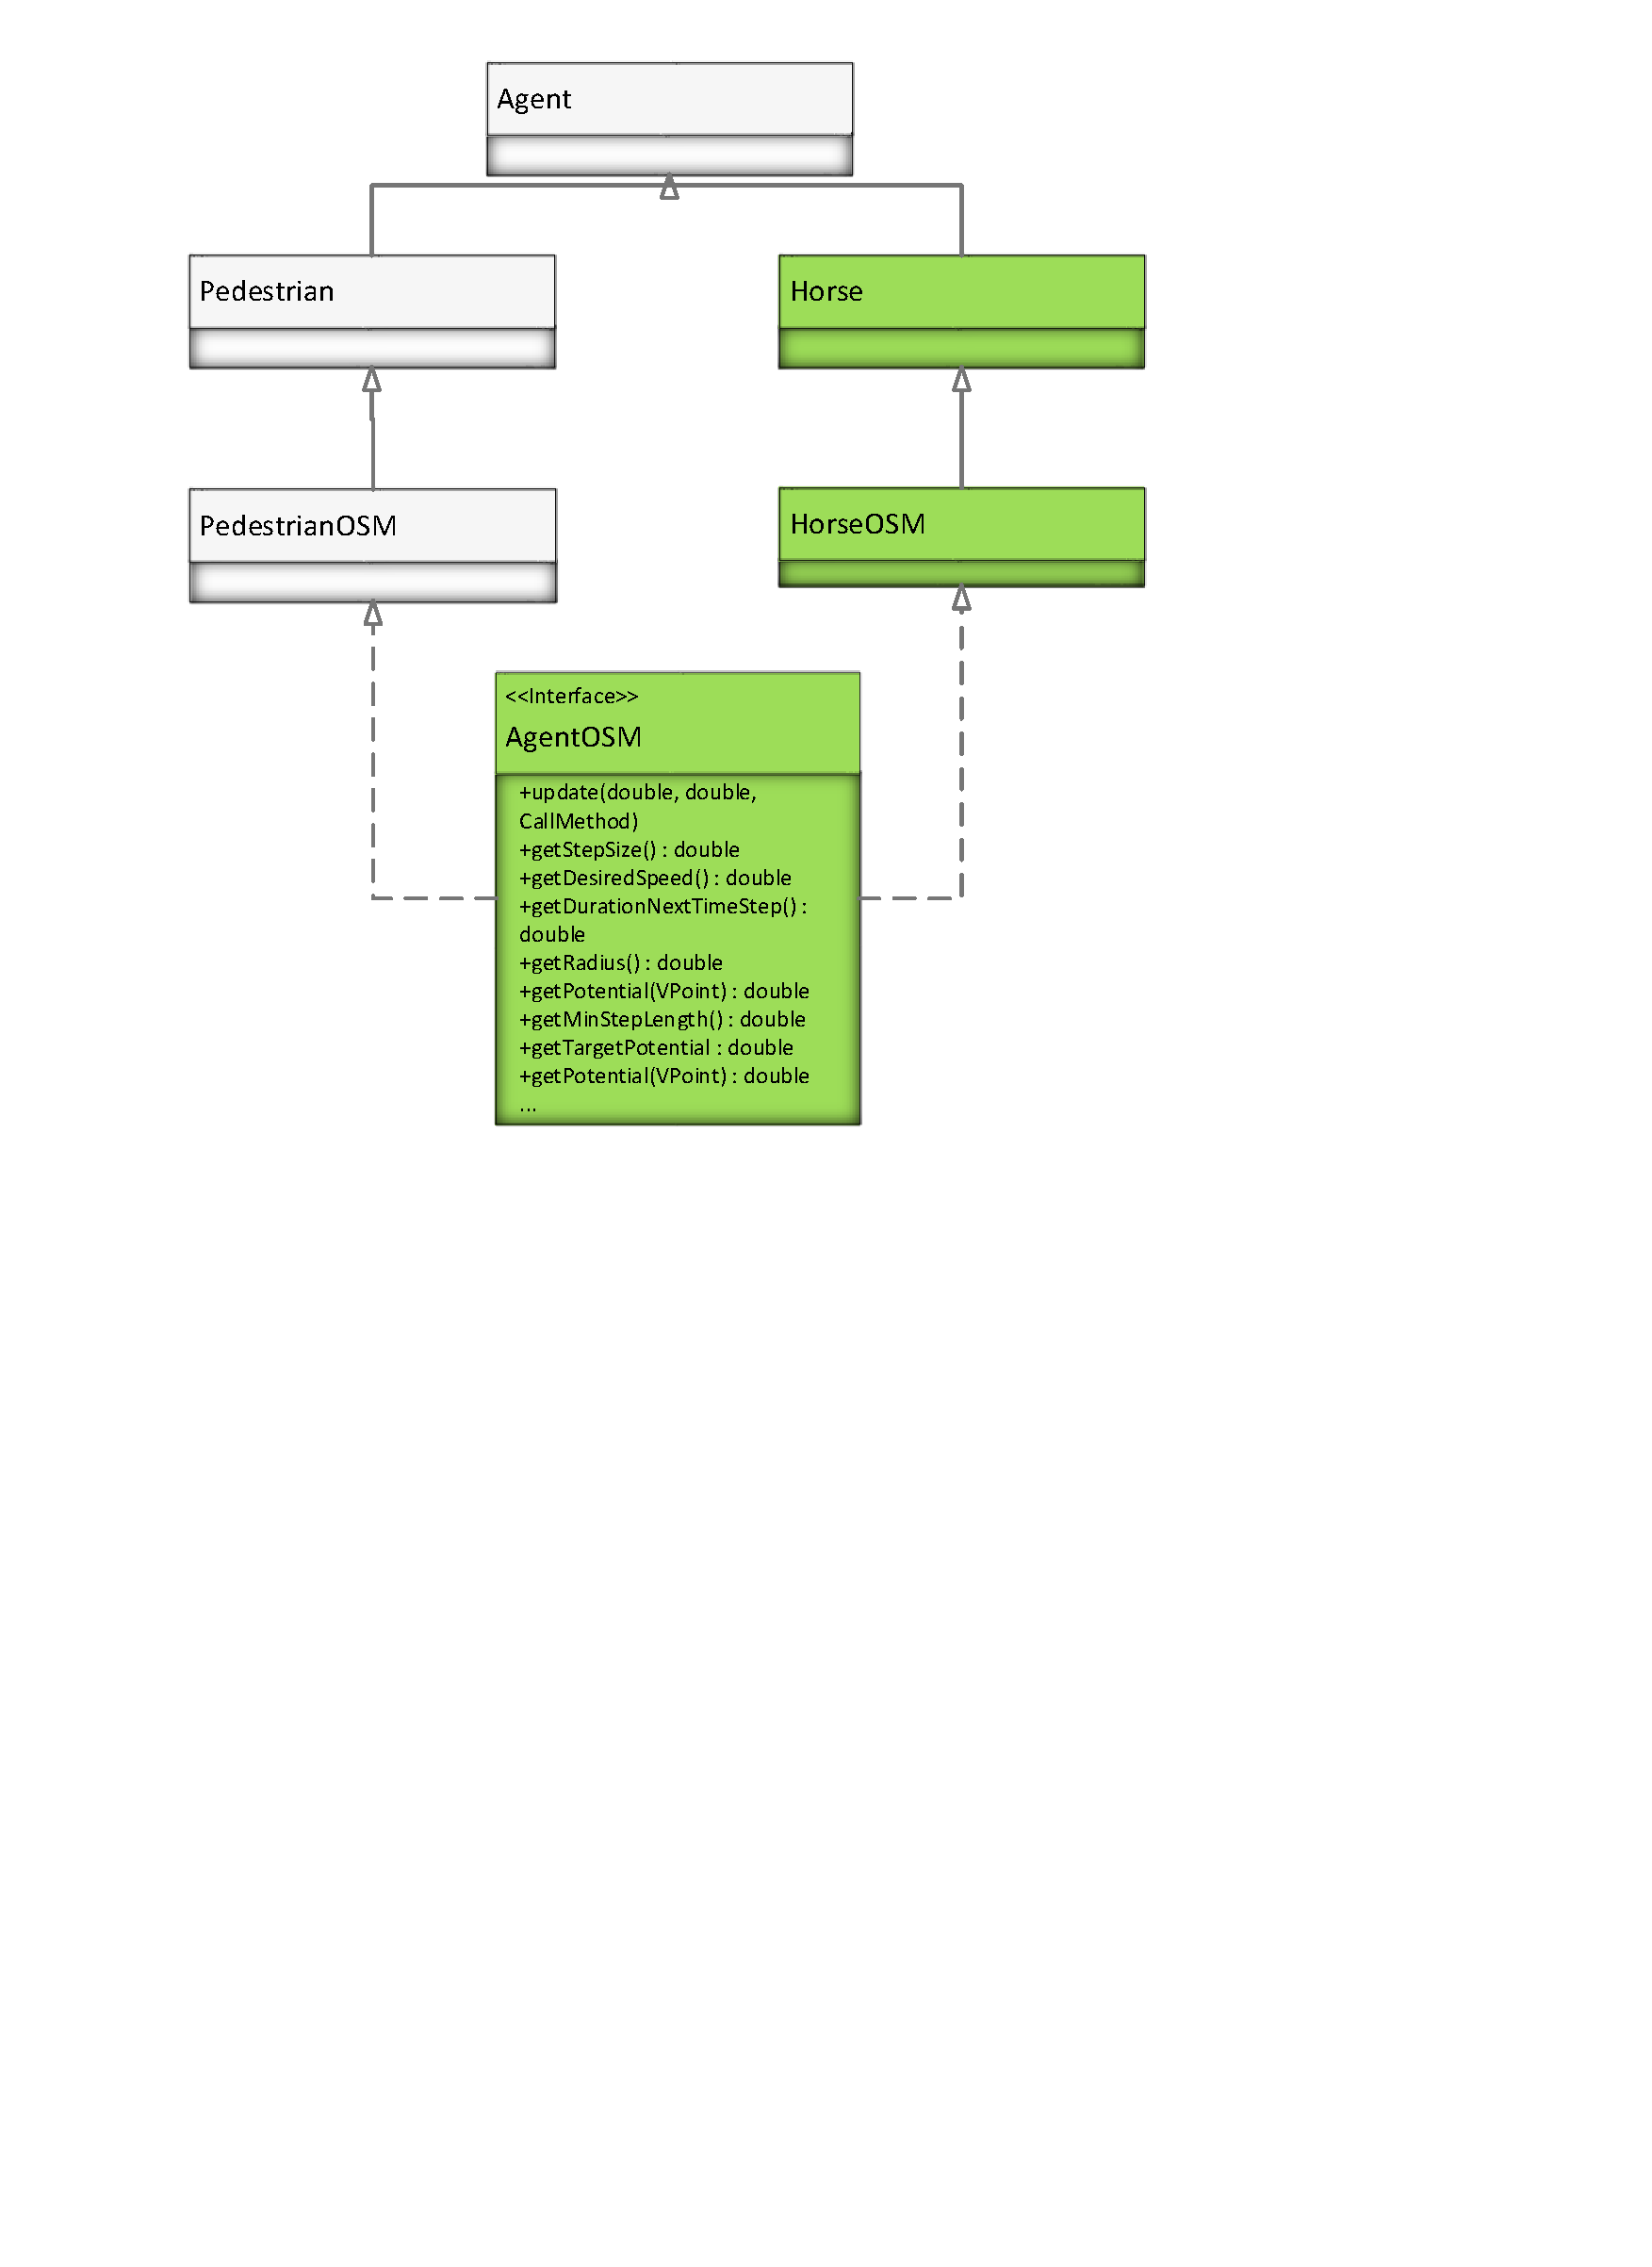
\includegraphics[width=\textwidth, keepaspectratio]{appendix/uml/OSM-nachher.pdf}
	\end{figure}
\end{frame}

\begin{frame}{Ein Schritt im OSM}
	\begin{figure}
		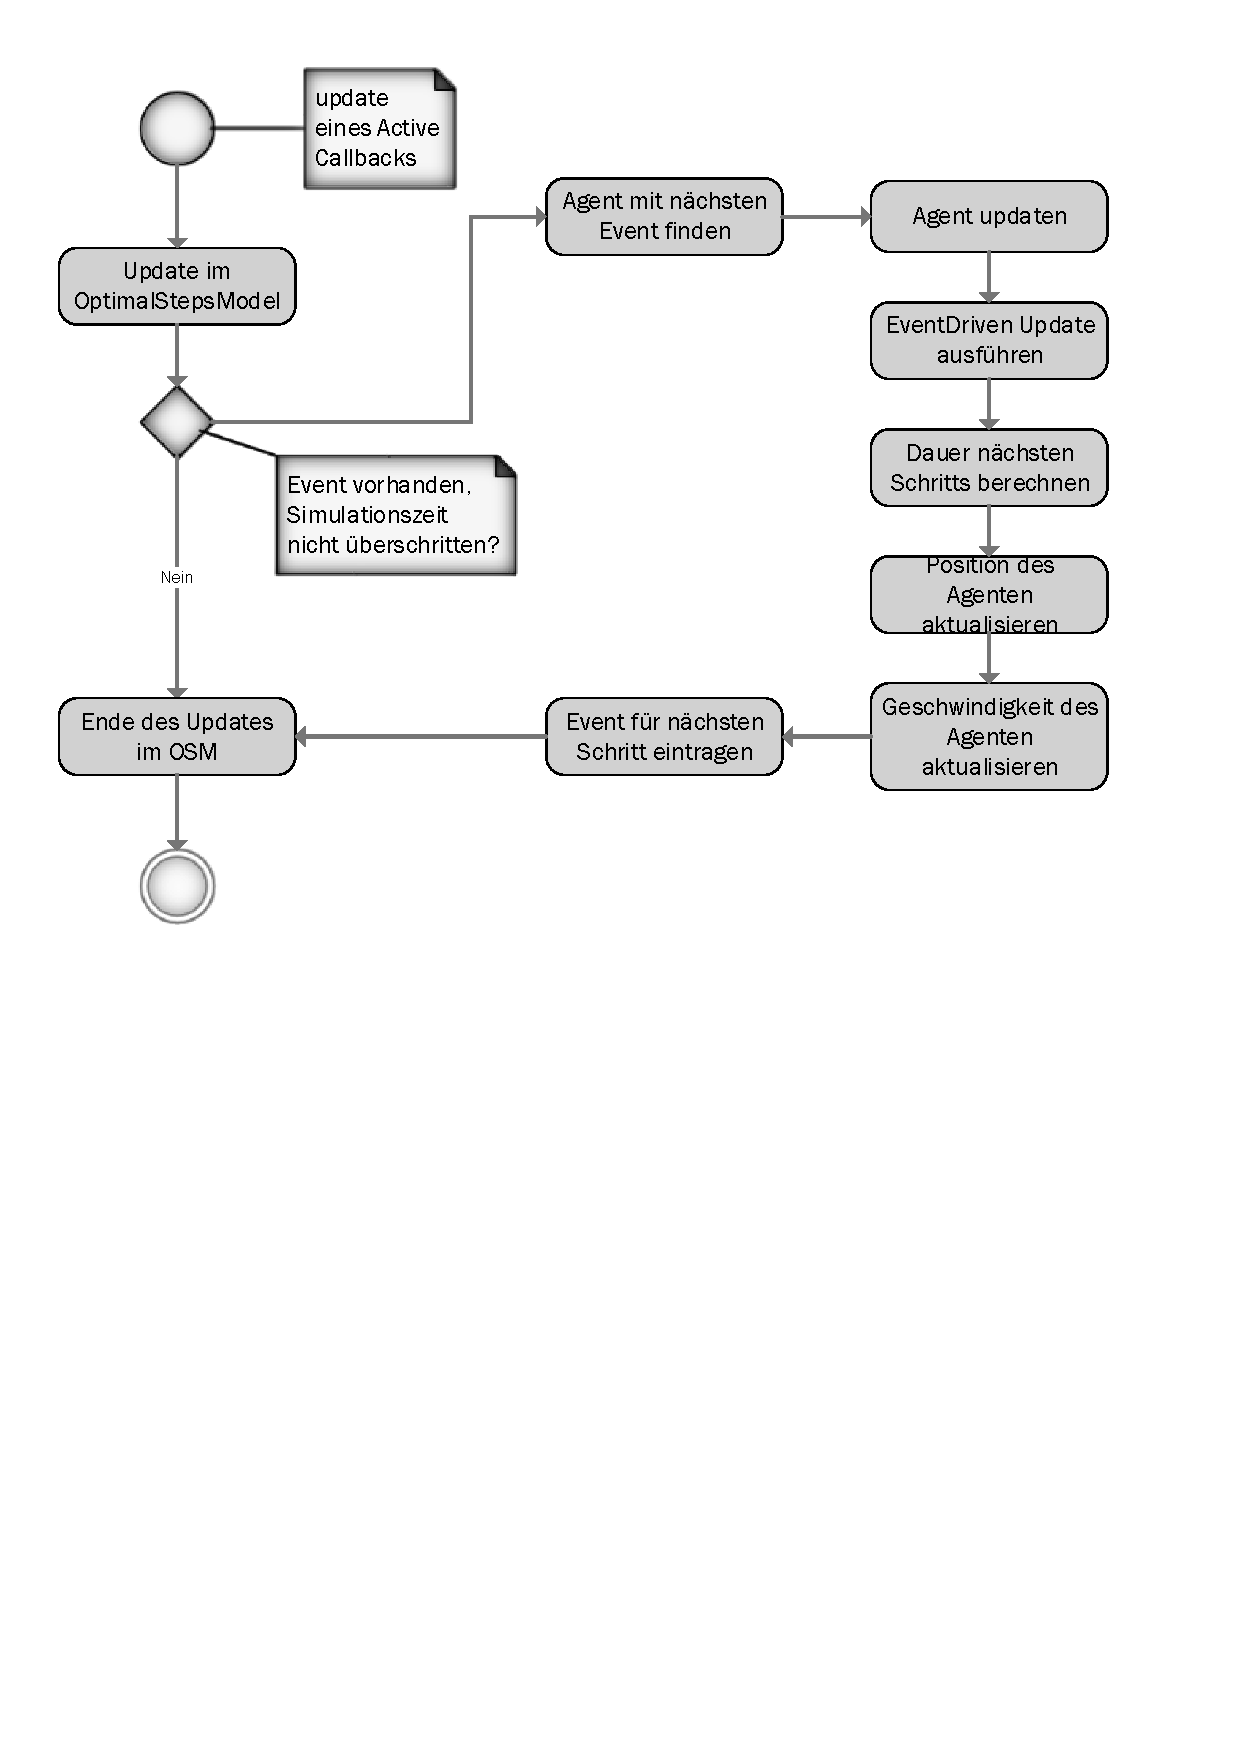
\includegraphics[width=\textwidth, keepaspectratio]{appendix/uml/EventDrivenUpdate.pdf}
	\end{figure}
\end{frame}

\begin{frame}{Fazit}
	Schwierigkeiten:
	\begin{itemize}
		\item Meine Arbeitszeiten
	\end{itemize}
	Fand ich gut:
	\begin{itemize}
		\item Organisation durch Trello, Skype
		\item Arbeitsaufteilung
		\item gutes Klima
		\item Anteil 19\%
	\end{itemize}
\end{frame}